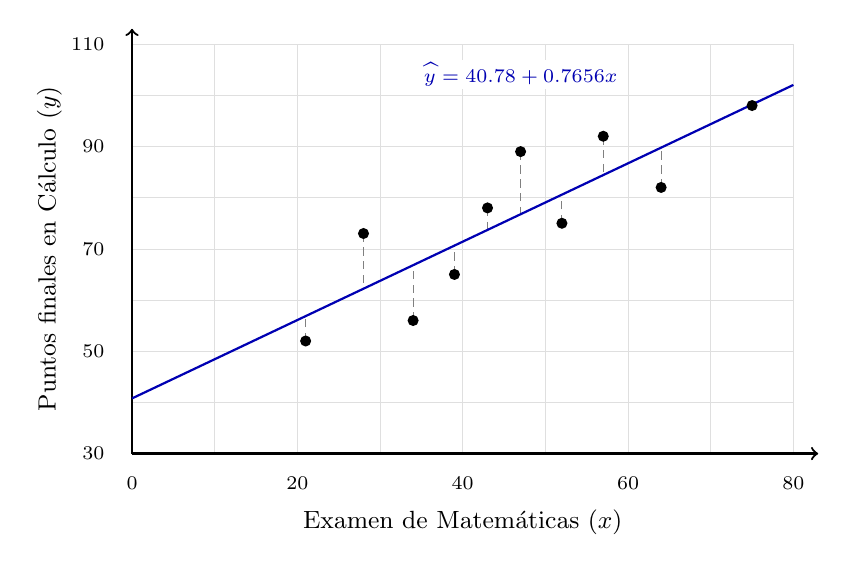
\begin{tikzpicture}[x=0.105cm,y=0.065cm]
    \draw[step=10,gray!25,very thin] (0,30) grid (80,110);
    \draw[->,thick] (0,30) -- (83,30);
    \draw[->,thick] (0,30) -- (0,113);
    \foreach \x in {0,20,40,60,80} {
        \node[below=2pt,font=\scriptsize] at (\x,28.5) {\x};
    }
    \foreach \y in {30,50,70,90,110} {
        \node[left=2pt,font=\scriptsize] at (-1.5,\y) {\y};
    }
    \node[below=14pt,font=\small] at (40,28.5) {Examen de Matemáticas ($x$)};
    \node[rotate=90,font=\small] at (-10,70) {Puntos finales en Cálculo ($y$)};
    \draw[gray,densely dashed] (39,65) -- (39,70.64);
    \draw[gray,densely dashed] (43,78) -- (43,73.70);
    \draw[gray,densely dashed] (21,52) -- (21,56.86);
    \draw[gray,densely dashed] (64,82) -- (64,89.78);
    \draw[gray,densely dashed] (57,92) -- (57,84.42);
    \draw[gray,densely dashed] (47,89) -- (47,76.77);
    \draw[gray,densely dashed] (28,73) -- (28,62.22);
    \draw[gray,densely dashed] (75,98) -- (75,98.20);
    \draw[gray,densely dashed] (34,56) -- (34,66.81);
    \draw[gray,densely dashed] (52,75) -- (52,80.59);
    \draw[blue!70!black,thick] (0,40.78) -- (80,102.03);
    \node[blue!70!black,fill=white,inner sep=1pt,font=\scriptsize] at (47,104) {$\widehat y=40.78+0.7656x$};
    \foreach \x/\y in {39/65,43/78,21/52,64/82,57/92,47/89,28/73,75/98,34/56,52/75} {
        \fill[black] (\x,\y) circle (2pt);
    }
\end{tikzpicture}